\documentclass[journal,12pt,onecolumn]{IEEEtran}
\usepackage{cite}
\usepackage{graphicx}
\usepackage{amsmath,amssymb,amsfonts,amsthm}
\usepackage{algorithmic}
\usepackage{graphicx}
\usepackage{textcomp}
\usepackage{xcolor}
\usepackage{txfonts}
\usepackage{listings}
\usepackage{enumitem}
\usepackage{mathtools}
\usepackage{gensymb}
\usepackage{comment}
\usepackage[breaklinks=true]{hyperref}
\usepackage{tkz-euclide} 
\usepackage{listings}
\usepackage{gvv}                                        
%\def\inputGnumericTable{}                                 
\usepackage[latin1]{inputenc} 
\usetikzlibrary{arrows.meta, positioning}
\usepackage{xparse}
\usepackage{color}                                            
\usepackage{array}                                            
\usepackage{longtable}                                       
\usepackage{calc}                                             
\usepackage{multirow}
\usepackage{multicol}
\usepackage{hhline}                                           
\usepackage{ifthen}                                           
\usepackage{lscape}
\usepackage{tabularx}
\usepackage{array}
\usepackage{float}
\newtheorem{theorem}{Theorem}[section]
\newtheorem{problem}{Problem}
\newtheorem{proposition}{Proposition}[section]
\newtheorem{lemma}{Lemma}[section]
\newtheorem{corollary}[theorem]{Corollary}
\newtheorem{example}{Example}[section]
\newtheorem{definition}[problem]{Definition}
\newcommand{\BEQA}{\begin{eqnarray}}
\newcommand{\EEQA}{\end{eqnarray}}
\usepackage{float}
%\newcommand{\define}{\stackrel{\triangle}{=}}
\theoremstyle{remark}
\usepackage{circuitikz}
\usepackage{tikz} % Required for inserting images
\graphicspath{{figs/}}
\usepackage{tfrupee}

\title{\textbf{GATE 2025 Statistics(ST)}}
\author{EE25BTECH11022 - sankeerthan}
\date{}

\begin{document}

\maketitle

\begin{enumerate}

\item Even though I had planned to go skiing with my friends, I had to \underline{\phantom{imagine}} at the last moment because of an injury.
Select the most appropriate option to complete the above sentence. \begin{enumerate}
\item back up
\item back of
\item back on
\item back out
\end{enumerate}
\hfill{(GATE ST 2025)}
\item The President, along with the Council of Ministers, \underline{\phantom{imagine}} to visit India next week.
Select the most appropriate option to complete the above sentence.
\begin{enumerate}
\item will wish
\item wishes
\item will wishes
\item is wishing
\end{enumerate}
\hfill{(GATE ST 2025)}
\item
An electricity utility company charges \rupee 7 per kWh (kilo watt-hour). If a 40-watt desk light is left on for 10 hours each night for 180 days, what would be the cost of energy consumption? If the desk light is on for 2 more hours each night for the 180 days, what would be the percentage-increase in the cost of energy consumption?

\begin{enumerate}
\item \rupee 604.8; 10\%
\item \rupee 504; 20\%
\item \rupee 604.8; 12\%
\item \rupee 720; 15\%
\end{enumerate}
\hfill{(GATE ST 2025)}
\item In the context of the given figure, which one of the following options correctly represents the entries in the blocks labelled (i), (ii), (iii), and (iv), respectively?

\begin{figure}
    \centering
    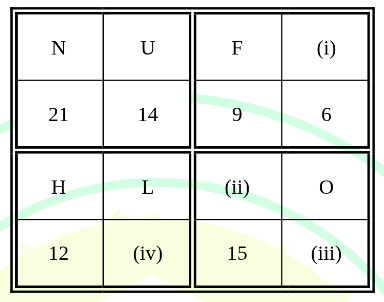
\includegraphics[width=0.3\columnwidth]{figs/7.png}
    \caption{}
    \label{fig:placeholder}
\end{figure}
\begin{enumerate}
\item Q, M, 12, and 8
\item K, L, 10 and 14
\item I, J, 10, and 8
\item L, K, 12 and 8
\end{enumerate}
\hfill{(GATE ST 2025)}
\item A bag contains Violet (V), Yellow (Y), Red (R), and Green (G) balls. On counting them, the following results are obtained: \\
(i) The sum of Yellow balls and twice the number of Violet balls is 50.\\
(ii) The sum of Violet and Green balls is 50.\\
(iii) The sum of Yellow and Red balls is 50.\\
(iv) The sum of Violet and twice the number of Red balls is 50.\\
Which one of the following Pie charts correctly represents the balls in the bag?
\begin{enumerate}

\item  \begin{figure}
    \centering
    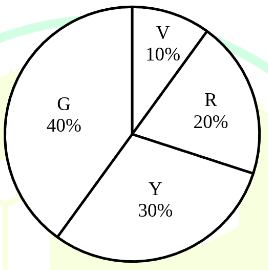
\includegraphics[width=0.5\columnwidth]{figs/1.png}
    \caption{}
    \label{fig:1}
\end{figure}

\item  \begin{figure}
    \centering
    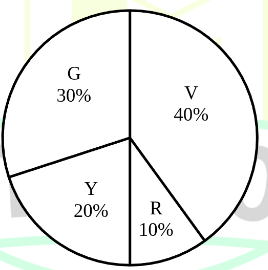
\includegraphics[width=0.5\columnwidth]{figs/2.png}
    \caption{}
    \label{fig:2}
\end{figure}

\item  \begin{figure}
    \centering
    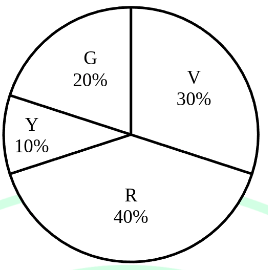
\includegraphics[width=0.5\columnwidth]{figs/3.png}
    \caption{}
    \label{fig:3}
\end{figure}

\item  \begin{figure}
    \centering
    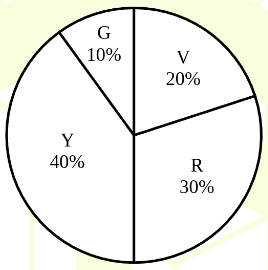
\includegraphics[width=0.5\columnwidth]{figs/4.png}
    \caption{}
    \label{fig:4}
\end{figure}

\end{enumerate}
\hfill{(GATE ST 2025)}
\newpage
\item ``His life was divided between the books, his friends, and long walks. A solitary man, he worked at all hours without much method, and probably courted his fatal illness in this way. To his own name there is not much to show; but such was his liberality that he was continually helping others, and fruits of his erudition are widely scattered, and have gone to increase many a comparative stranger's reputation.''
(From E.V. Lucas's ``A Funeral'')
Based only on the information provided in the above passage, which one of the following statements is true?
\begin{enumerate}
\item The solitary man described in the passage is dead.
\item Strangers helped create a grand reputation for the solitary man described in the passage.
\item The solitary man described in the passage found joy in scattering fruits.
\item The solitary man worked in a court where he fell ill.
\end{enumerate}
\hfill{(GATE ST 2025)}
\newpage
\item For the clock shown in the figure, if $O^* = OQSZPRT$, and $X^* = XZPWYOQ$, then which one among the given options is most appropriate for $P^*$?

\begin{figure}
    \centering
    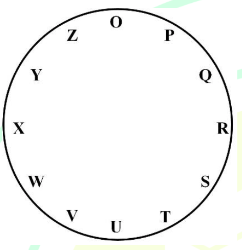
\includegraphics[width=0.2\columnwidth]{figs/5.png}
    \caption{}
    \label{fig:placeholder}
\end{figure}
\begin{enumerate}
\item PUWRTVX
\item PRTO QSU
\item PTVQSUW
\item PSUPRTV
\end{enumerate}
\hfill{(GATE ST 2025)}
\item Consider a five-digit number PQRST that has distinct digits P, Q, R, S, and T, and satisfies the following conditions: $P<Q$, $S>P>T$, $R<T$. If integers 1 through 5 are used to construct such a number, the value of P is: \begin{enumerate}
\item 1
\item 2
\item 3
\item 4
\end{enumerate}
\hfill{(GATE ST 2025)}
\item A business person buys potatoes of two different varieties P and Q, mixes them in a certain ratio and sells them at \rupee 192 per kg. The cost of variety P is \rupee 800 for 5 kg. The cost of variety Q is \rupee 800 for 4 kg. If the person gets 8\% profit, what is the P:Q ratio (by weight)?    \begin{enumerate}
\item 5:4
\item 3:4
\item 3:2
\item 1:1
\end{enumerate}
\hfill{(GATE ST 2025)}
\newpage
\item Three villages P, Q, and R are located in such a way that the distance $PQ = 13$ km, $QR = 14$ km, and $RP = 15$ km, as shown in the figure. A straight road joins Q and R. It is proposed to connect P to this road QR by constructing another road. What is the minimum possible length (in km) of this connecting road?
\begin{figure}
    \centering
    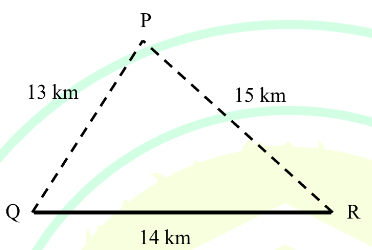
\includegraphics[width=0.2\columnwidth]{figs/6.png}
    \caption{}
    \label{fig:6}
\end{figure}
\begin{enumerate}
\item 10.5
\item 11.0
\item 12.0
\item 12.5
\end{enumerate}
\hfill{(GATE ST 2025)}
\item Let $f: \lsbrak{0},\rbrak{\infty} \rightarrow\lsbrak{0},\rbrak{\infty}$ be a differentiable function with $f\brak{x} > 0$ for all $x > 0$, and $f\brak{0} = 0$. Further, $f$ satisfies
$
\brak{f\brak{x}}^2 = \int_{0}^{x} \brak{\brak{f\brak{t}}^2 + f\brak{t}}\, dt, \quad x > 0.
$
Then which one of the following options is correct?
\begin{enumerate}
\item $0 < f\brak{2} \leq 1$
\item $1 < f\brak{2} \leq 2$
\item $2 < f\brak{2} \leq 3$
\item $3 < f\brak{2} \leq 4$
\end{enumerate}
\hfill{(GATE ST 2025)}
\item Among the following four statements about countability and uncountability of different sets, which is the correct statement?
\begin{enumerate}
\item The set $U_{n=0}\brak{x\in \mathbb{R}: x = \sum_{i=0}^n 10^{-i} a_i,\, a_i\in\brak{1,2}}$ is uncountable.
\item The set $\brak{x\in\brak{0,1}:x=\sum_{n=1}^{\infty} a_n/10^n,\, a_n=1\textrm{ or }2,\, n\in\mathbb{N}}$ is uncountable.
\item There exists an uncountable set whose elements are pairwise disjoint open intervals in $\mathbb{R}$.
\item The set of all intervals with rational end points is uncountable.
\end{enumerate}
\hfill{(GATE ST 2025)}
\item Let $S = \brak{\brak{x, y, z} \in \mathbb{R}^3 \setminus \cbrak{\brak{0,0,0}} : z = -\brak{x + y} }$. Denote
$
S^+ =\brak{\brak{p,q,r} \in \mathbb{R}^3 : px + qy + rz = 0 \text{ for all } \brak{x, y, z} \in S}.
$
Then which one of the following options is correct?
\begin{enumerate}
\item $S^+$ is not a subspace of $\mathbb{R}^3$
\item $S^+ = \cbrak{\brak{0,0,0}}$
\item $\dim\brak{S^+} = 1$
\item $\dim\brak{S^+} = 2$
\end{enumerate}
\hfill{(GATE ST 2025)}
\item Let $X$ be a random variable having the Poisson distribution with mean $\log_e2$. Then $\mathbb{E}\brak{e^{\brak{\log_e3X}}}$ equals
\begin{enumerate}
\item 1
\item 2
\item 3
\item 4
\end{enumerate}
\hfill{(GATE ST 2025)}
\item Let $\brak{X_1, X_2, X_3}$ follow the multinomial distribution with the number of trials being 100 and the probability vector $\brak{\frac{1}{3}, \frac{1}{3}, \frac{1}{3}}$. Then $\mathbb{E}\brak{X_2|X_3=40}$ equals
\begin{enumerate}
\item 25
\item 15
\item 30
\item 45
\end{enumerate}
\hfill{(GATE ST 2025)}
\item Let $\brak{X_n}_{n\geq1}$ be a sequence of i.i.d. random variables with the common probability density function
$
f\brak{x}=\frac{1}{\pi\brak{1+x^2}},~-\infty < x < \infty.
$
Define $Y_n = \frac{1}{n}\sum_{i=1}^n \tan^{-1}\brak{X_i}$ for $n = 1,2,\ldots$.
Then which one of the following options is correct?
\begin{enumerate}
\item $P\brak{\sum_{i=1}^n Y_i/n \to 2 \text{ as } n\rightarrow\infty}=1$
\item $P\brak{\sum_{i=1}^n Y_i/n \to 0 \text{ as } n\rightarrow\infty}=1$
\item $P\brak{\sum_{i=1}^n Y_i \to 0 \text{ as } n\rightarrow\infty}=1$
\item $P\brak{\frac{1}{n}\sum_{i=1}^n X_i \to \infty \text{ as } n\rightarrow\infty}=1$
\end{enumerate}
\hfill{(GATE ST 2025)}
\item Let $\brak{N\brak{t}: t \geq 0}$ be a homogenous Poisson process with the intensity/rate $\lambda = 2$. Let $X = N\brak{6} - N\brak{1}$, $Y = N\brak{5} - N\brak{3}$, $W = N\brak{6} - N\brak{5}$, $Z = N\brak{3} - N\brak{1}$.
Then which one of the following options is correct?
\begin{enumerate}
\item $\operatorname{Cov}\brak{W,Z} = 2$
\item $Y + Z \sim \operatorname{Poisson}\brak{10}$
\item $\Pr\brak{Y = Z} = 1$
\item $\operatorname{Cov}\brak{X,Y} = 4$
\end{enumerate}
\hfill{(GATE ST 2025)}
\item Let $T$ be a complete and sufficient statistic for a family $\mathcal{P}$ of distributions and let $U$ be a sufficient statistic for $\mathcal{P}$. If $P_f(T>0) = 1$ for all $f\in\mathcal{P}$, then which one of the following options is NOT necessarily correct?
\begin{enumerate}
\item $T^2$ is a complete statistic for $\mathcal{P}$
\item $T^2$ is a minimal sufficient statistic for $\mathcal{P}$
\item $T$ is a function of $U$
\item $U$ is a function of $T$
\end{enumerate}
\hfill{(GATE ST 2025)}
\item Let $X_1, X_2$ be a random sample from $N\brak{0,1}$ distribution, where $\theta\in\mathbb{R}$. Consider testing $H_0: \theta=0$ against $H_1:\theta \neq 0$. Let $\Phi\brak{X_1, X_2}$ be the likelihood ratio test of size 0.05 for testing $H_0$ against $H_1$. Then which one of the following options is correct?
\begin{enumerate}
\item $\brak{X_1, X_2}$ is a uniformly most powerful test of size 0.05
\item $E_\theta(\Phi\brak{X_1,X_2}) \geq 0.05~\forall\theta \in \mathbb{R}$
\item There exists a uniformly most powerful test of size 0.05
\item $E_{\theta=0}\brak{X_1\Phi\brak{X_1,X_2}} = 0.05$
\end{enumerate}
\hfill{(GATE ST 2025)}
\item Let a random variable $X$ follow a distribution with density $f\in\brak{f_0, f_1}$, where
$f_0\brak{x}=1, \, 0\leq x\leq 1,~0$ otherwise;
$f_1\brak{x}=1, \, 1\leq x\leq 2,~0$ otherwise.
Let $\phi$ be a most powerful test of level 0.05 for testing $H_0: f=f_0$ against $H_1: f=f_1$ based on $X$. Then which one of the following options is necessarily correct?
\begin{enumerate}
\item $E_{f_0}\brak{\phi\brak{x}} = 0.05$
\item $E_{f_1}\brak{\phi\brak{x}} = 1$
\item $P_f\brak{\phi\brak{x} = 1} = P_f\brak{X > 1}, \forall f \in\brak{f_0, f_1}$
\item $P_{f_1}\brak{\phi\brak{x} = 1} < 1$
\end{enumerate}
\hfill{(GATE ST 2025)}
\item Let $X$ have pdf $f \in \brak{f_0,f_1}$. Let $\varphi$ be a most powerful test of level $0.05$ for testing $H_0:f=f_0$ against $H_1:f=f_1$ based on $X$. Which one is NOT necessarily correct?

\begin{enumerate}
\item $\varphi$ is the unique most powerful test of level $0.05$
\item $E_{f_1}(\varphi\brak{x}) \geq 0.05$
\item $E_{f_0}(\varphi\brak{x}) \leq 0.05$
\item For some constant $c\geq 0$, 
$P_f\!\brak{ \frac{f_1\brak{x}}{f_0\brak{x}} > c } \leq P_f\brak{\varphi\brak{x}=1}, \; \forall f\in \brak{f_0,f_1}$
\end{enumerate}
\hfill{(GATE ST 2025)}

\item Let $\brak{X_n}_{n\geq 1}$ be i.i.d. with cdf $F$. Let $F_n$ be the empirical cdf. For fixed $x\in \mathbb{R}$:
\begin{enumerate}
\item $\sqrt{n}\brak{F_n\brak{x}-F\brak{x}} \xrightarrow{P} 0$
\item $n\brak{F_n\brak{x}-F\brak{x}} \xrightarrow{d} Z \sim N\big(0, F\brak{x}(1-F\brak{x})\big)$
\item $\lim_{n\to\infty} n\operatorname{Var}\brak{F_n\brak{x}} = 0$
\item $\sqrt{n}\brak{F_n\brak{x}-F\brak{x}} \xrightarrow{d} Z \sim N\brak{0, F\brak{x}\brak{1-F\brak{x}}}$
\end{enumerate}
\hfill{(GATE ST 2025)}
\item Let $\brak{X,Y}$ follow a bivariate normal with
$
E\brak{x}=3,\quad E\brak{Y}=4,\quad \mathrm{Var}\brak{x}=25,\quad \mathrm{Var}\brak{Y}=100,\quad \mathrm{Cov}\brak{X,Y}=50\rho.
$
If $E\brak{Y|X=5}=4.32$, then $\rho$ equals
\begin{enumerate}
\item $0.08$
\item $0.8$
\item $0.32$
\item $0.5$
\end{enumerate}
\hfill{(GATE ST 2025)}
\item For data $\brak{x_i,y_i}$, $i=1,\dots,n$ with $\sum x_i>0$, let
$
\hat{\beta} = \arg\min_{\beta\in \mathbb{R}} \sum_{i=1}^n \brak{y_i - \beta x_i}^2.
$
Define $v_j = y_j-x_j$, $u_j = 2x_j$, and let 
$
\hat{\gamma} = \arg\min_{\gamma\in \mathbb{R}} \sum_{i=1}^n \brak{v_i - \gamma u_i}^2.
$
If $\hat{\beta}=10$, then $\hat{\gamma}=$
\begin{enumerate}
\item $4.5$ \item $5$ \item $10$ \item $9$
\end{enumerate}
\hfill{(GATE ST 2025)}
\item Let
$
I=\int_0^1 \int_0^1 y^2 \cos\brak{\pi\brak{1+xy}}   dx  dy .
$
The value of $I$ is \underline{\phantom{imagine}} (integer).
\hfill{(GATE ST 2025)}
\item Let 
$P=\myvec{ 2 & -1 \\ -1 & 4 }$, 
$Q=P^3 - 2P^2 -4P + 13I_2$.  
Then $\det\brak{Q}=$ \underline{\phantom{imagine}} (integer).
\hfill{(GATE ST 2025)}
\item Let $T:\mathbb{R}^3\to\mathbb{R}^3$ be defined by
$
T\brak{x_1,x_2,x_3} = \brak{3x_1+5x_2+x_3,\; x_3,\; 2x_1+2x_3}.
$
The rank of $T$ is \underline{\phantom{imagine}} (integer).
\hfill{(GATE ST 2025)}
\item Let $X$ have cdf $F$ with
$\lim_{h\to 0^-} F\brak{3+h}=\tfrac{1}{4}$, and $F\brak{3}=\tfrac{3}{4}$.
Then $16\,Pr\brak{X=3}=$ \underline{\phantom{imagine}} (integer).
\hfill{(GATE ST 2025)}
\item Let $X\sim Bin\brak{2,\tfrac{2}{3}}$. Then $18E\brak{X^2}=$ \underline{\phantom{imagine}} (integer).
\hfill{(GATE ST 2025)}
\item Let $X\in \mathbb{R}^{10} \sim N\brak{0,I_{10}}$. Define $Y=\log\!\sqrt{X^T X}$. Let $M_Y\brak{t}$ be its mgf. Then $M_Y\brak{2}=$ \underline{\phantom{imagine}} (integer).
\hfill{(GATE ST 2025)}
\item If $\brak{W\brak{t}}$ is standard Brownian motion, then $E\brak{\brak{W\brak{2}+W\brak{3}}^2}=$ \underline{\phantom{imagine}} (integer).
\hfill{(GATE ST 2025)}
\item A sample of size 5 from $Bin\brak{1,\theta}$ with $\theta\in \lbrak{0},\rsbrak{0.7}$ gives observations $0,1,1,1,0$. The MLE of $\theta$ is \underline{\phantom{imagine}}.
\hfill{(GATE ST 2025)}
\item Let $X_1,\dots,X_5 \sim N\brak{0,\theta}$ i.i.d. Then the Cramér--Rao lower bound $c\brak{\theta}$ for unbiased estimators of $\theta$ has $\inf_\theta c\brak{\theta}=$ \underline{\phantom{imagine}} (integer).
\hfill{(GATE ST 2025)}
\item Sample data $\brak{1,3},\brak{2,4},\brak{7,8}$. The Spearman rank correlation is \underline{\phantom{imagine}} (two decimal places).
\hfill{(GATE ST 2025)}
\item In regression
$
Y_i=\beta_0+\beta_1X_{1i}+\beta_2X_{2i}+\beta_3X_{3i}+\beta_4X_{4i}+\epsilon_i, \quad i=1,\dots,25,
$
with $\epsilon_i\sim N\brak{0,\sigma^2}$, suppose $R^2=0.5$. Then adjusted-$R^2=$ \underline{\phantom{imagine}} (two decimals).
\hfill{(GATE ST 2025)}
\item Let $F=\brak{f:\sbrak{a,b}\to \mathbb{R} \mid f \text{ continuous on }\sbrak{a,b}, f' \text{ exists on }\brak{a,b}}$. Which is correct?
\begin{enumerate}
\item There exists non-constant $f\in F$ with $|f\brak{x}-f\brak{y}|\leq |x-y|^2,\,\forall x,y\in \sbrak{a,b}$
\item If $f\in F$ and $x_0\in\brak{a,b}$, there exist distinct $x_1,x_2$ with 
$\dfrac{f\brak{x_1}-f\brak{x_2}}{x_1-x_2}=f'(x_0)$
\item If $f'\brak{x}\geq 0$ and $f'$ vanishes only at two points, then $f$ is strictly increasing
\item If $f'\brak{x_1}<c<f'\brak{x_2}$ for some $x_1<x_2$, then there may NOT exist $x_0\in\brak{x_1,x_2}$ with $f'\brak{x_0}=c$
\end{enumerate}
\hfill{(GATE ST 2025)}
\item Over $U=\brak{\brak{X,Y}: x+y\leq 2}$, minimize $f\brak{X,Y}=(x-1)^4+(y-2)^4$. The minimum is
\begin{enumerate}
\item $1/16$
\item $7$
\item $17/81$
\item $1/8$
\end{enumerate}
\hfill{(GATE ST 2025)}
\item Let $P=\brak{a_{ij}}_{10\times 10}$ with 
$a_{ij}=\tfrac{1}{10}$ if $i\neq j$, and $a_{ii}=\tfrac{9}{10}$. Then $\mathrm{rank}\brak{P}=$
\begin{enumerate}
\item 10 \item 9 \item 1 \item 8
\end{enumerate}
\hfill{(GATE ST 2025)}
\item Let $X$ with cdf
$
F\brak{x}=
0,  x<0, \\
\alpha\brak{1+2x^2},  0<x<1, \\
1,  x\geq 1.
$
If median of $X$ is $\tfrac{1}{2}$, then $\alpha=$
\begin{enumerate}
\item $2/13$ \item $1$ \item $1/4$ \item $1/6$
\end{enumerate}
\hfill{(GATE ST 2025)}
\item If $X$ has lognormal pdf:
$
f\brak{x} = \frac{1}{\sigma x \sqrt{2\pi}} \exp\!\brak{-\frac{(\ln x -\mu)^2}{2\sigma^2}}, \quad x>0,
$
with $\mu\in\mathbb{R}, \sigma>0$. If $\ln \brak{E\brak{X^2}}=4$, then $\mathrm{Var}\brak{\ln X}=$
\begin{enumerate}
\item 2 \item 4 \item 16 \item 64
\end{enumerate}
\hfill{(GATE ST 2025)}

\item Let $X$ and $Y$ be discrete random variables with joint probability mass function  
$
p_{X,Y}\brak{m,n}= \frac{\lambda^n e^{-\lambda}}{2^n m! \brak{n-m})!}, \quad m = 0, \dots, n,\; n = 0,1,2,\dots
$  
where $\lambda$ is a fixed positive real number. Then which one of the following options is correct?
\begin{enumerate}
\item The marginal distribution of $X$ is Poisson with mean $\lambda$
\item The marginal distribution of $Y$ is Poisson with mean $2\lambda$
\item The conditional distribution of $X$ given $Y=3$ is $\text{Bin}\brak{3,\tfrac{1}{2}}$
\item $E\brak{Y|X=2} = \tfrac{\lambda}{2}$
\end{enumerate}
\hfill{(GATE ST 2025)}
\item Let $X_1,\dots,X_n, \; n \geq 2,$ be a random sample from a $N\brak{-\theta,\theta}$ distribution, where $\theta>0$ is an unknown parameter. Then which one of the following options is correct?
\begin{enumerate}
\item $\sum_{i=1}^n X_i$ is a minimal sufficient statistic
\item $\sum_{i=1}^n X_i^2$ is a minimal sufficient statistic
\item $\brak{ \tfrac{1}{n}\sum_{i=1}^n X_i,\; \tfrac{1}{n-1}\sum_{j=1}^n \brak{X_j - \tfrac{1}{n}\sum_{i=1}^n X_i}^2}$ is a complete statistic
\item $-\tfrac{1}{n}\sum_{i=1}^n X_i$ is a uniformly minimum variance unbiased estimator of $\theta$
\end{enumerate}
\hfill{(GATE ST 2025)}
\item Let $X_1,X_2$ be a random sample from a distribution with density
$
f_\theta\brak{x} = 
\tfrac{1}{\theta} e^{-x/\theta},  x>0 \\
0,  \text{otherwise},
$
where $\theta>0$ is unknown. For testing $H_0:\theta\leq 1$ vs $H_1:\theta>1$, consider the test
$
\phi\brak{X_1,X_2} = 
1,  X_1>1 \\
0,  \text{otherwise}.
$
Then which one of the following tests has the same power function as $\phi$?
\begin{enumerate}
\item $\phi_1\brak{X_1,X_2} = \frac{X_1+X_2-1}{X_1+X_2}, \;\; \text{if } X_1+X_2>1, \; 0 \text{ otherwise}$
\item $\phi_2\brak{X_1,X_2} = \frac{2X_1+2X_2-1}{2\brak{X_1+X_2}}, \;\; \text{if } X_1+X_2>1, \; 0 \text{ otherwise}$
\item $\phi_3\brak{X_1,X_2} = \frac{3X_1+3X_2-1}{3\brak{X_1+X_2}}, \;\; \text{if } X_1+X_2>1, \; 0 \text{ otherwise}$
\item $\phi_4\brak{X_1,X_2} = \frac{4X_1+4X_2-1}{4\brak{X_1+X_2}}, \;\; \text{if } X_1+X_2>1, \; 0 \text{ otherwise}$
\end{enumerate}
\hfill{(GATE ST 2025)}
\item Let $X,Y_1,Y_2$ be independent random variables such that $X$ has pdf  
$
f\brak{x} = 
2e^{-2x},  x \geq 0, \\
0,  \text{otherwise},
$
and $Y_1,Y_2$ are i.i.d. with pdf
$
g\brak{x} = 
e^{-x},  x \geq 0, \\
0,  \text{otherwise}.
$
For $i=1,2$, let $R_i$ denote the rank of $Y_i$ among $X,Y_1,Y_2$. Then $E\brak{R_1+R_2}$ equals
\begin{enumerate}
\item $13/3$
\item $22/5$
\item $21/5$
\item $9/2$
\end{enumerate}
\hfill{(GATE ST 2025)}
\item Let $X_1,\dots,X_5$ be i.i.d. random vectors following the bivariate normal distribution with zero mean vector and identity covariance matrix. Define the $5 \times 2$ matrix $X = \brak{X_1,\dots,X_5}^T$. Further, let $W=\brak{W_{ij}}=X^TX$, and $Z=W_{11}+4W_{12}+4W_{22}$. Then $\text{Var}\brak{Z}$ equals

\begin{enumerate}
\item 150
\item 200
\item 250
\item 300
\end{enumerate}
\hfill{(GATE ST 2025)}
\item Consider the simple linear regression model
$
y_i = \alpha + \beta x_i + \epsilon_i, \quad i=1,2,\dots,24,
$
where $\alpha,\beta \in \mathbb{R}$ are unknown, and $\epsilon_i$ are i.i.d. $N(0,\sigma^2)$ with $\sigma>0$. Suppose the following summary statistics are obtained:
$
S_{xx} = \sum_{i=1}^{24}\brak{x_i-\bar{x}}^2 = 22.82, \quad 
S_{yy} = \sum_{i=1}^{24}\brak{y_i-\bar{y}}^2 = 43.62,
$
$
S_{xy} = \sum_{i=1}^{24}\brak{x_i-\bar{x}}\brak{y_i-\bar{y}} = 15.48,
$
where $\bar{x}=\tfrac{1}{24}\sum_{i=1}^{24} x_i$, $\;\bar{y}=\tfrac{1}{24}\sum_{i=1}^{24} y_i$.  
For testing $H_0:\beta=0$ against $H_1:\beta \neq 0$, the value of the $F$-test statistic (with distribution $F_{1,22}$) equals (rounded off to two decimals):
\begin{enumerate}
\item 2.54
\item 2.98
\item 3.17
\item 6.98
\end{enumerate}
\hfill{(GATE ST 2025)}
\item Let $\brak{x_n}_{n\geq 1}$ be defined as
$
x_n = 1 + \frac{1}{\sqrt{2}} + \frac{1}{\sqrt{3}} + \cdots + \frac{1}{\sqrt{n}} - 2\brak{\sqrt{n}-1}.
$
Which of the following options is/are correct?
\begin{enumerate}
\item The sequence $\brak{x_n}_{n\geq 1}$ is unbounded
\item The sequence $\brak{x_n}_{n\geq 1}$ is monotonically decreasing
\item The sequence $\brak{x_n}_{n\geq 1}$ is bounded but does not converge
\item The sequence $\brak{x_n}_{n\geq 1}$ converges
\end{enumerate}
\hfill{(GATE ST 2025)}
\item Let $\mathcal{O} = \cbrak{P: P \text{ is a } 3\times 3 \text{ real matrix with } P^TP=I_3, \det\brak{P}=1}$.  
Which of the following options is/are correct?
\begin{enumerate}
\item There exists $P \in \mathcal{O}$ with $\lambda=\tfrac{1}{2}$ as an eigenvalue
\item There exists $P \in \mathcal{O}$ with $\lambda=2$ as an eigenvalue
\item If $\lambda$ is the only real eigenvalue of $P \in \mathcal{O}$, then $\lambda=1$
\item There exists $P \in \mathcal{O}$ with $\lambda=-1$ as an eigenvalue
\end{enumerate}
\hfill{(GATE ST 2025)}
\item Let $X_1,X_2,X_3$ be independent standard normal random variables, and define
$
Y_1=X_1-X_2, \quad Y_2=X_1+X_2-2X_3, \quad Y_3=X_1+X_2+X_3.
$
Which of the following options is/are correct?
\begin{enumerate}
\item $Y_1,Y_2,Y_3$ are independent
\item $Y_1^2+Y_2^2+Y_3^2 \sim \chi^2_3$
\item $\dfrac{2Y_3}{\sqrt{3Y_1^2+Y_2^2}} \sim t_2$
\item $\dfrac{3Y_1^2+2Y_3^2}{2Y_2^2} \sim F_{1,1}$
\end{enumerate}
\hfill{(GATE ST 2025)}
\item Let $\brak{x_n}_{n\geq 1}$ be independent random variables with $X_n \xrightarrow{\text{a.s.}} 0$ as $n \to \infty$.  
Which of the following options is/are necessarily correct?
\begin{enumerate}
\item $E\brak{X_n^3} \to 0$ as $n\to\infty$
\item $X_n^7 \xrightarrow{P} 0$ as $n\to\infty$
\item For any $\epsilon>0$, $\sum_{n=1}^\infty \Pr\brak{|X_n|\geq \epsilon}<\infty$
\item $X_n^2+X_n+5 \xrightarrow{\text{a.s.}} 5$ as $n\to\infty$
\end{enumerate}
\hfill{(GATE ST 2025)}
\item Consider a Markov chain $\cbrak{X_n:n=1,2,\dots}$ with state space $S=\cbrak{1,2,3}$ and transition probability matrix
$
P=\myvec{
0 & 1/2 & 1/2 \\
1/3 & 0 & 2/3 \\
2/5 & 3/5 & 0
}.
$
Define $\pi=\brak{\tfrac{18}{67},\tfrac{24}{67},\tfrac{25}{67}}$. Which of the following options is/are correct?
\begin{enumerate}
\item $\pi$ is a stationary distribution of $P$
\item $\pi^T$ is an eigenvector of $P^T$
\item $\Pr\brak{X_3=1|X_1=1}=\tfrac{11}{30}$
\item At least one state is transient
\end{enumerate}
\hfill{(GATE ST 2025)}
\item Let $X_1,\dots,X_n$ be a random sample from $\text{Uniform}\brak{-\tfrac{\theta}{2},\tfrac{\theta}{2}}$, where $\theta>0$. Which of the following options is/are correct?
\begin{enumerate}
\item $2\max\cbrak{X_1,\dots,X_n}$ is the maximum likelihood estimator of $\theta$
\item $\brak\min\cbrak{X_1,\dots,X_n}, \max\cbrak{X_1,\dots,X_n})$ is a sufficient statistic
\item $\brak{min\cbrak{X_1,\dots,X_n}, \max\cbrak{X_1,\dots,X_n}}$ is a complete statistic
\item $\dfrac{2\brak{n+1}}{n}\max\{|X_1|,\dots,|X_n|\}$ is a UMVUE of $\theta$
\end{enumerate}
\hfill{(GATE ST 2025)}
\item Let $X=\brak{X_1,X_2,X_3}^T$ have a $N_3\brak{0,\Sigma}$ distribution with
$
\Sigma = \myvec{
4 & 0 & 0 \\
0 & 9 & 0 \\
0 & 0 & 4
}.
$
Let $\alpha^T=\brak{2,0,-1}$ and $\beta^T=\brak{1,1,1}$. Which of the following statements is/are correct?
\begin{enumerate}
\item $E\brak{\text{trace}\brak{XX^T\alpha\alpha^T}}=20$
\item $\text{Var}\brak{\text{trace}\brak{X\alpha^T}}=20$
\item $E\brak{\text{trace}\brak{XX^T}}=17$
\item $\text{Cov}\brak{\alpha^TX,\beta^TX}=3$
\end{enumerate}
\hfill{(GATE ST 2025)}
\item For $Y\in\mathbb{R}^n$, $X\in\mathbb{R}^{n\times p}$, $\beta\in\mathbb{R}^p$, consider the regression model
$
Y=X\beta+\epsilon,
$
where $\epsilon\sim N_n\brak{0,I_n}$. For $\lambda>0$, define
$
\hat{\beta}_n=\brak{X^TX+\lambda I_p}^{-1}X^TY.
$
Which of the following options is/are correct?
\begin{enumerate}
\item $\hat{\beta}_n$ is an unbiased estimator of $\beta$
\item $\brak{X^TX+\lambda I_p}$ is positive definite
\item $\hat{\beta}_n$ has a multivariate normal distribution
\item $\text{Var}(\hat{\beta}_n)=\brak{X^TX+\lambda I_p}^{-1}$
\end{enumerate}
\hfill{(GATE ST 2025)}
\item Let $f:\mathbb{R}^2\to\mathbb{R}$ be defined as $f\brak{x,y}=x^2y^2+8x-4y$. The number of saddle points of $f$ is \underline{\phantom{imagine}} (answer in integer).

\item[Q.56] Let  
$
P=\myvec{
0 & 1 & 1 & 1 & 1 \\
-1 & 0 & 1 & 1 & 1 \\
-1 & -1 & 0 & 1 & 1 \\
-1 & -1 & -1 & 0 & 1 \\
-1 & -1 & -1 & -1 & 0
}.
$
If $\lambda_1,\lambda_2,\lambda_3,\lambda_4,\lambda_5$ are eigenvalues of $P$, then $\prod_{i=1}^5 \lambda_i =$ \underline{\phantom{imagine}} (answer in integer).
\hfill{(GATE ST 2025)}
\item Let  
$
P=\myvec{2 & 1 \\ 1 & 2}, 
\quad 
Q=\myvec{1 & 1 \\ -2 & 4}.
$
Then $\text{trace}\brak{P^5+Q^4}=$ \underline{\phantom{imagine}} (answer in integer).
\hfill{(GATE ST 2025)}
\item The moment generating functions of three independent random variables $X,Y,Z$ are given by
$
M_X\brak{t}=\tfrac{1}{9}\brak{2+e^t}^2, \quad
M_Y\brak{t}=e^{\brak{e^t-1}}, \quad
M_Z\brak{t}=e^{2\brak{e^t-1}}, \quad t\in\mathbb{R}.
$
Then $10\Pr\brak{X>Y+Z}=$ \underline{\phantom{imagine}} (rounded off to two decimal places).
\hfill{(GATE ST 2025)}
\item The service times (in minutes) at two petrol pumps $P_1$ and $P_2$ follow distributions with pdfs
$
f_1\brak{x}=\lambda e^{-\lambda x}, \; x>0,
\quad 
f_2\brak{x}=\lambda^2 x e^{-\lambda x}, \; x>0,
$
where $\lambda>0$. For service, a customer chooses $P_1$ or $P_2$ randomly with equal probability. Suppose the probability that the service time exceeds one minute is $2e^{-2}$. Then $\lambda=$ \underline{\phantom{imagine}} (answer in integer).
\hfill{(GATE ST 2025)}
\item Let $\brak{x_n}_{n\geq 1}$ be independent random variables with
$
\Pr\!\brak{X_n=-\tfrac{1}{2^n}} = \Pr\!\brak{X_n=\tfrac{1}{2^n}}=\tfrac{1}{2}, \quad n\in\mathbb{N}.
$
Suppose $\sum_{i=1}^n X_i \xrightarrow{d} U$ as $n\to\infty$. Then $6\Pr\brak{U\leq \tfrac{2}{3}}=$ \underline{\phantom{imagine}} (answer in integer).
\hfill{(GATE ST 2025)}
\item Let $X_1,\dots,X_7$ be a random sample from a population with pdf
$
f\brak{x}=\tfrac{1}{2}\lambda^3 x^2 e^{-\lambda x}, \quad x>0,
$
where $\lambda>0$ is unknown. Let $\hat{\lambda}$ be the MLE of $\lambda$, and $E\brak{\hat{\lambda}-\lambda}=\alpha\lambda$ be the bias, with $\alpha$ a constant. Then $\tfrac{1}{\alpha}=$ \underline{\phantom{imagine}} (answer in integer).
\hfill{(GATE ST 2025)}
\item Let $X_1,X_2$ be a random sample from a population with pdf
$
f_\theta\brak{x}=
e^{x-\theta},  -\infty < x \leq \theta, \\
0,  \text{otherwise},
$
where $\theta\in\mathbb{R}$. Consider testing $H_0:\theta\geq 0$ against $H_1:\theta<0$ at level $\alpha=0.09$. Let $\beta\brak{\theta}$ be the power function of a UMP test. Then $\beta\brak{\log 0.36}=$ \underline{\phantom{imagine}} (rounded off to two decimal places).
\hfill{(GATE ST 2025)}
\item Let $X\sim \text{Bin}\brak{3,\theta}$, $\theta\in\brak{0,1}$. For testing  
$H_0:\tfrac{1}{4}\leq \theta \leq \tfrac{3}{4}$ against $H_1:\theta<\tfrac{1}{4}$ or $\theta>\tfrac{3}{4}$, consider
$
\phi\brak{x}=
1,  x\in\cbrak{0,3}, \\
0,  x\in\cbrak{1,2}.
$
The size of $\phi$ is \underline{\phantom{imagine}} (rounded off to two decimal places).
\hfill{(GATE ST 2025)}
\item Let $\brak{X_1,X_2,X_3}^T \sim N_3\!\brak{\myvec{0\\0\\0},
\myvec{
1 & 0.4 & 0 \\
0.4 & 1 & 0.6 \\
0 & 0.6 & 1
}}.
$
Then the partial correlation coefficient between $X_1$ and $X_2$ given $X_3$ is \underline{\phantom{imagine}} (rounded off to two decimal places).
\hfill{(GATE ST 2025)}
\item Let $(X,Y)^T$ follow a bivariate normal distribution with $E\brak{x}=2$, $E(Y)=3$, $\text{Var}\brak{x}=16$, $\text{Var}(Y)=25$, $\text{Cov}(X,Y)=14$. Then
$
2\pi\Big(\Pr(X>2,\;Y>3)-\tfrac{1}{4}\Big)
$
equals \underline{\phantom{imagine}} (rounded off to two decimal places).
\hfill{(GATE ST 2025)}
\end{enumerate}

\end{document}
